\documentclass[pdf]{beamer}
\mode<presentation>

\usetheme{CambridgeUS}

\usepackage[utf8]{inputenc}
\usepackage[T1]{fontenc}
\usepackage{setspace}
\usepackage{color}
\usepackage{listings}

\usepackage{minted}
\newminted{scala}{
    breaklines,
    fontsize=\scriptsize}

\newminted{proto}{
    breaklines,
    fontsize=\scriptsize}

\title[SparkNet]{SparkNet}
\subtitle{Training Deep Networks in Spark \cite{moritz2015sparknet}}
\author{Feynman Liang}
\institute{CUED}
\date{\today}

\begin{document}

\section{Introduction}

\begin{frame}
    \vfill
    \centering
    \begin{beamercolorbox}[sep=8pt,center,shadow=true,rounded=true]{title}
        \usebeamerfont{title}SMT Presentations: Computation\par%
    \end{beamercolorbox}
    \vfill
\end{frame}

\begin{frame}[t]{Motivation}
    \begin{columns}
        \begin{column}{0.49\textwidth}
            \begin{block}{Big data}
                \begin{figure}[htpb]
                    \centering
                    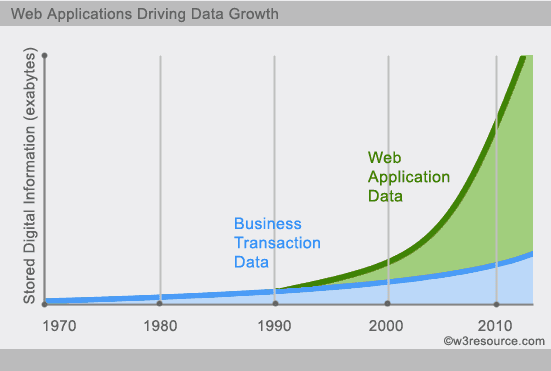
\includegraphics[width=\linewidth]{Figures/growing-data.png}
                \end{figure}
            \end{block}
        \end{column}
        \begin{column}{0.49\textwidth}
            \begin{block}{Cloud computing}
                \begin{figure}[htpb]
                    \centering
                    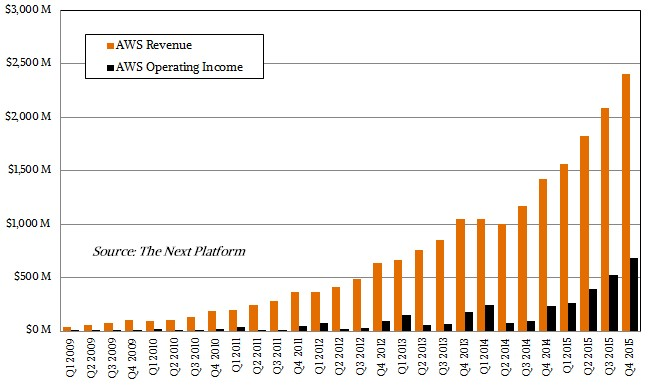
\includegraphics[width=\linewidth]{Figures/growing-cloud.jpg}
                \end{figure}
            \end{block}
        \end{column}
    \end{columns}

    \begin{block}{Problem}
        Datasets no longer fit on a single machine!
    \end{block}
\end{frame}

\begin{frame}[t]{Distributed Computing}
    \begin{columns}
        \begin{column}{0.7\textwidth}
            \begin{figure}[htpb]
                \centering
                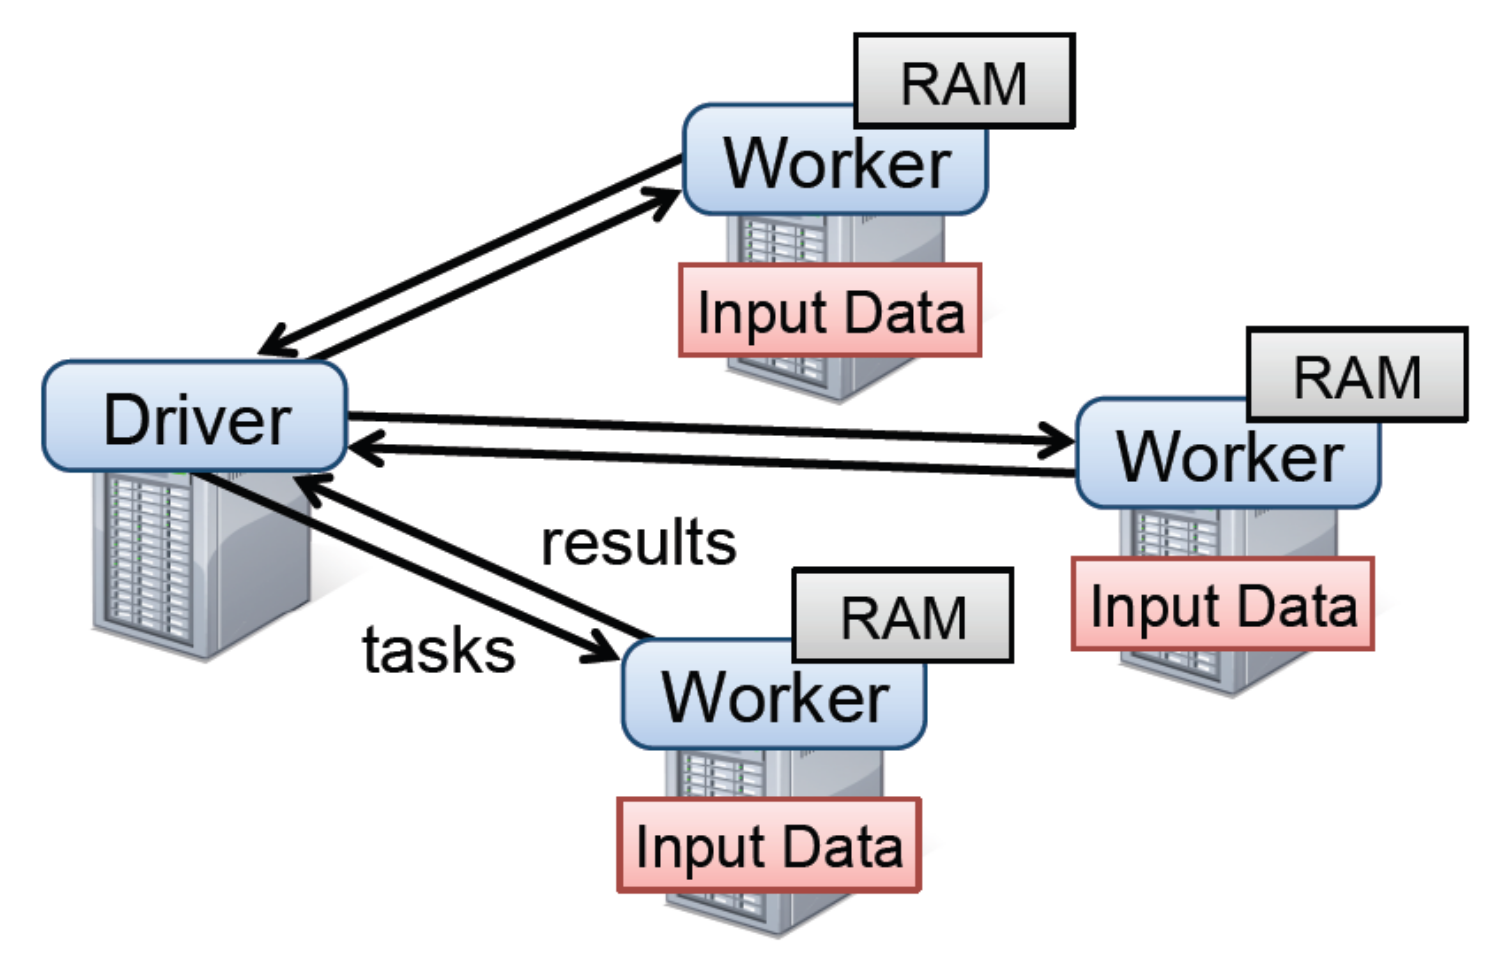
\includegraphics[width=\linewidth]{Figures/distcomp.png}
            \end{figure}
        \end{column}
        \begin{column}{0.3\textwidth}
            New concerns:
            \begin{enumerate}
                \item Consistency
                \item Availability
                \item Partition tolerance
            \end{enumerate}
            \begin{block}{CAP Theorem \cite{gilbert2002brewer}}
                Choose two
            \end{block}
        \end{column}
    \end{columns}
\end{frame}

\begin{frame}{MapReduce \cite{dean2008mapreduce}}
    \begin{columns}
        \begin{column}{0.3\textwidth}
            \begin{itemize}
                \item Job-level dependency tracking
                \item Disk I/O every iteration
            \end{itemize}
        \end{column}
        \begin{column}{0.7\textwidth}
            \begin{figure}[htpb]
                \centering
                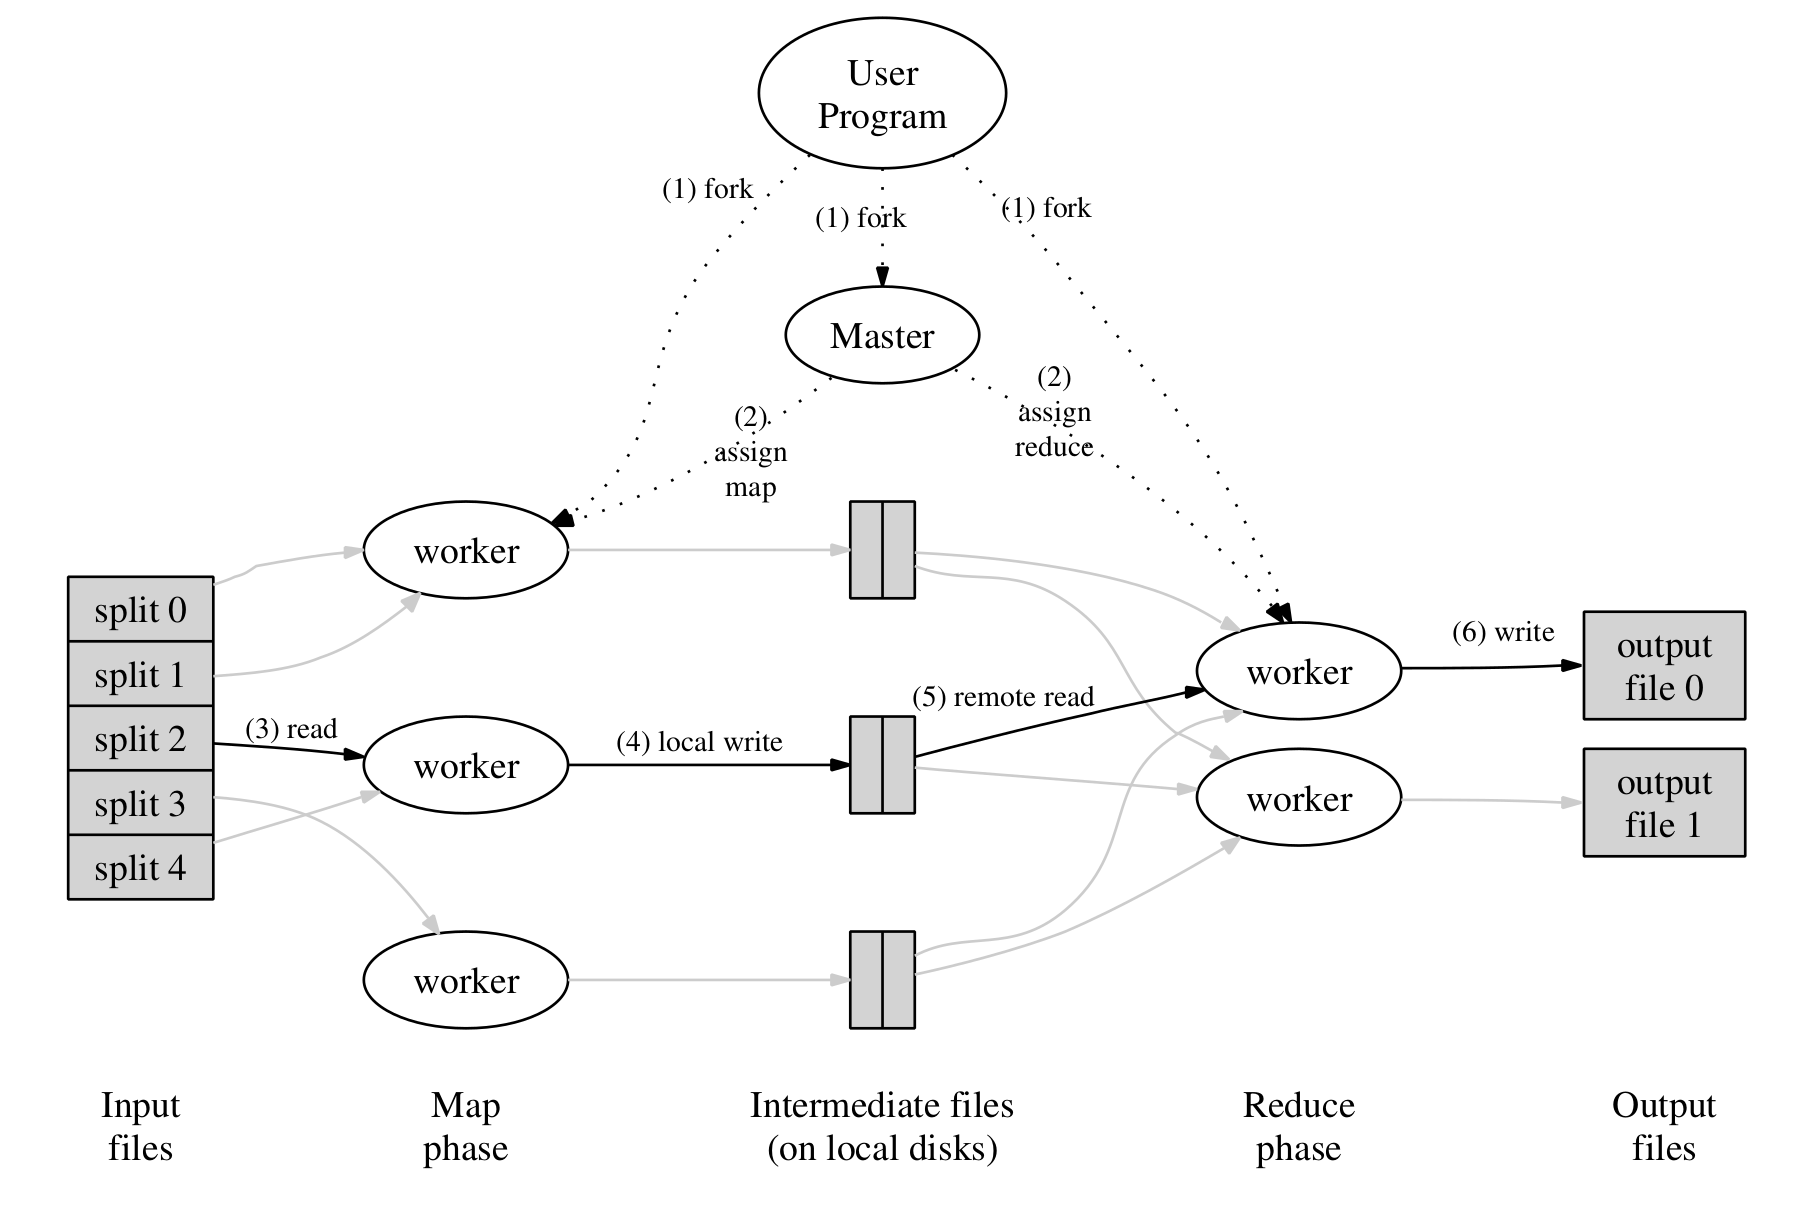
\includegraphics[width=\linewidth]{Figures/mapreduce.png}
            \end{figure}
        \end{column}
    \end{columns}
\end{frame}


\section{SparkNet}

\begin{frame}
    \titlepage
\end{frame}

\begin{frame}{Goals}
    \begin{itemize}
        \item ``Our goal is \textbf{not to outperform custom computational
            frameworks} but rather to propose a system that can be \textbf{easily
            implemented in popular batch frameworks} and that performs
            nearly as well\ldots''
        \item ``\ldots integration with a fast and general engine for big data
            processing such as Spark \textbf{allows researchers and practitioners
            to draw from a rich ecosystem of tools to develop and deploy
            their models}''
        \item ``In SparkNet, \textbf{training a deep network on the output of a SQL
            query, or a graph computation, or a streaming data source} is
            straightforward''
    \end{itemize}
\end{frame}

\section{Architecture Overview}

\begin{frame}[fragile]{Caffe \cite{jia2014caffe}}
    \begin{columns}
        \begin{column}{0.3\textwidth}
            \begin{itemize}
                \item Separation of concerns
                    \begin{itemize}
                        \item Model specification
                        \item Solver
                        \item CPU$\leftrightarrow$GPU
                    \end{itemize}
                \item Model Zoo
                \item GPU parallelism
            \end{itemize}
        \end{column}
        \begin{column}{0.25\textwidth}
            \begin{minted}[fontsize=\tiny]{proto}
name: "LogReg"
layer {
  name: "mnist"
  type: "Data"
  top: "data"
  top: "label"
  data_param {
    source: "input_leveldb"
    batch_size: 64
  }
}
layer {
  name: "ip"
  type: "InnerProduct"
  bottom: "data"
  top: "ip"
  inner_product_param {
    num_output: 2
  }
}
layer {
  name: "loss"
  type: "SoftmaxWithLoss"
  bottom: "ip"
  bottom: "label"
  top: "loss"
}
            \end{minted}
        \end{column}
        \begin{column}{0.35\textwidth}
            \begin{figure}[htpb]
                \centering
                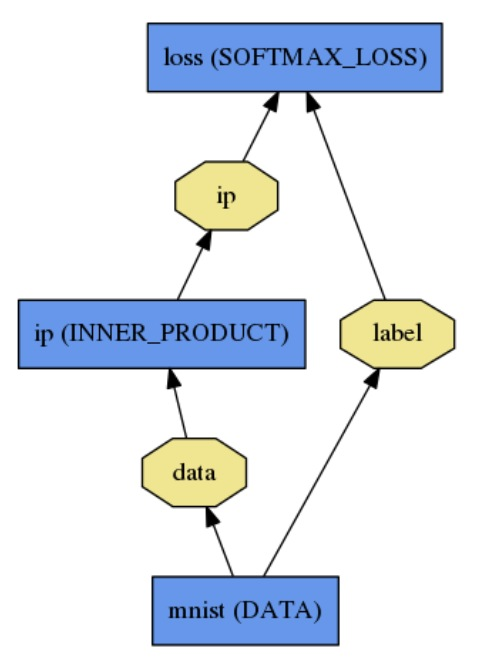
\includegraphics[width=\linewidth]{Figures/logreg}
            \end{figure}
        \end{column}
    \end{columns}
\end{frame}

\begin{frame}[fragile]{SparkNet's \mintinline{scala}{Net} API}
    Java Native Access (JNA) wrapper around Caffe

    \begin{scalacode}
class Net {
    def Net(netParams: NetParams): Net
    def setTrainingData(data: Iterator[(NDArray,Int)])
    def setValidationData(data: Iterator[(NDArray,Int)])
    def train(numSteps: Int)
    def test(numSteps: Int): Float
    def setWeights(weights: WeightCollection)
    def getWeights(): WeightCollection
}
    \end{scalacode}
\end{frame}

\begin{frame}[fragile]{Example CNN \mintinline{scala}{NetParams}}
    Compiled to \texttt{protobuf} Caffe network specification
    \begin{scalacode}
val netParams = NetParams(
    RDDLayer("data", shape=List(batchsize, 1, 28, 28)),
    RDDLayer("label", shape=List(batchsize, 1)),
    ConvLayer("conv1", List("data"), kernel=(5,5), numFilters=20),
    PoolLayer("pool1", List("conv1"), pool=Max, kernel=(2,2), stride=(2,2)),
    ConvLayer("conv2", List("pool1"), kernel=(5,5), numFilters=50),
    PoolLayer("pool2", List("conv2"), pool=Max, kernel=(2,2), stride=(2,2)),
    LinearLayer("ip1", List("pool2"), numOutputs=500),
    ActivationLayer("relu1", List("ip1"), activation=ReLU),
    LinearLayer("ip2", List("relu1"), numOutputs=10),
    SoftmaxWithLoss("loss", List("ip2", "label"))
)
    \end{scalacode}
\end{frame}

\begin{frame}{Spark \cite{zaharia2012resilient}}
    \begin{block}{Resilient Distributed Datasets (RDDs)}
        \begin{enumerate}
            \item \emph{Lineage graph} describing lazy dataset
            \item Aggressive in-memory caching (project Tungsten)
            \item Partition-level dependency tracking
        \end{enumerate}
    \end{block}
    \begin{figure}[htpb]
        \centering
        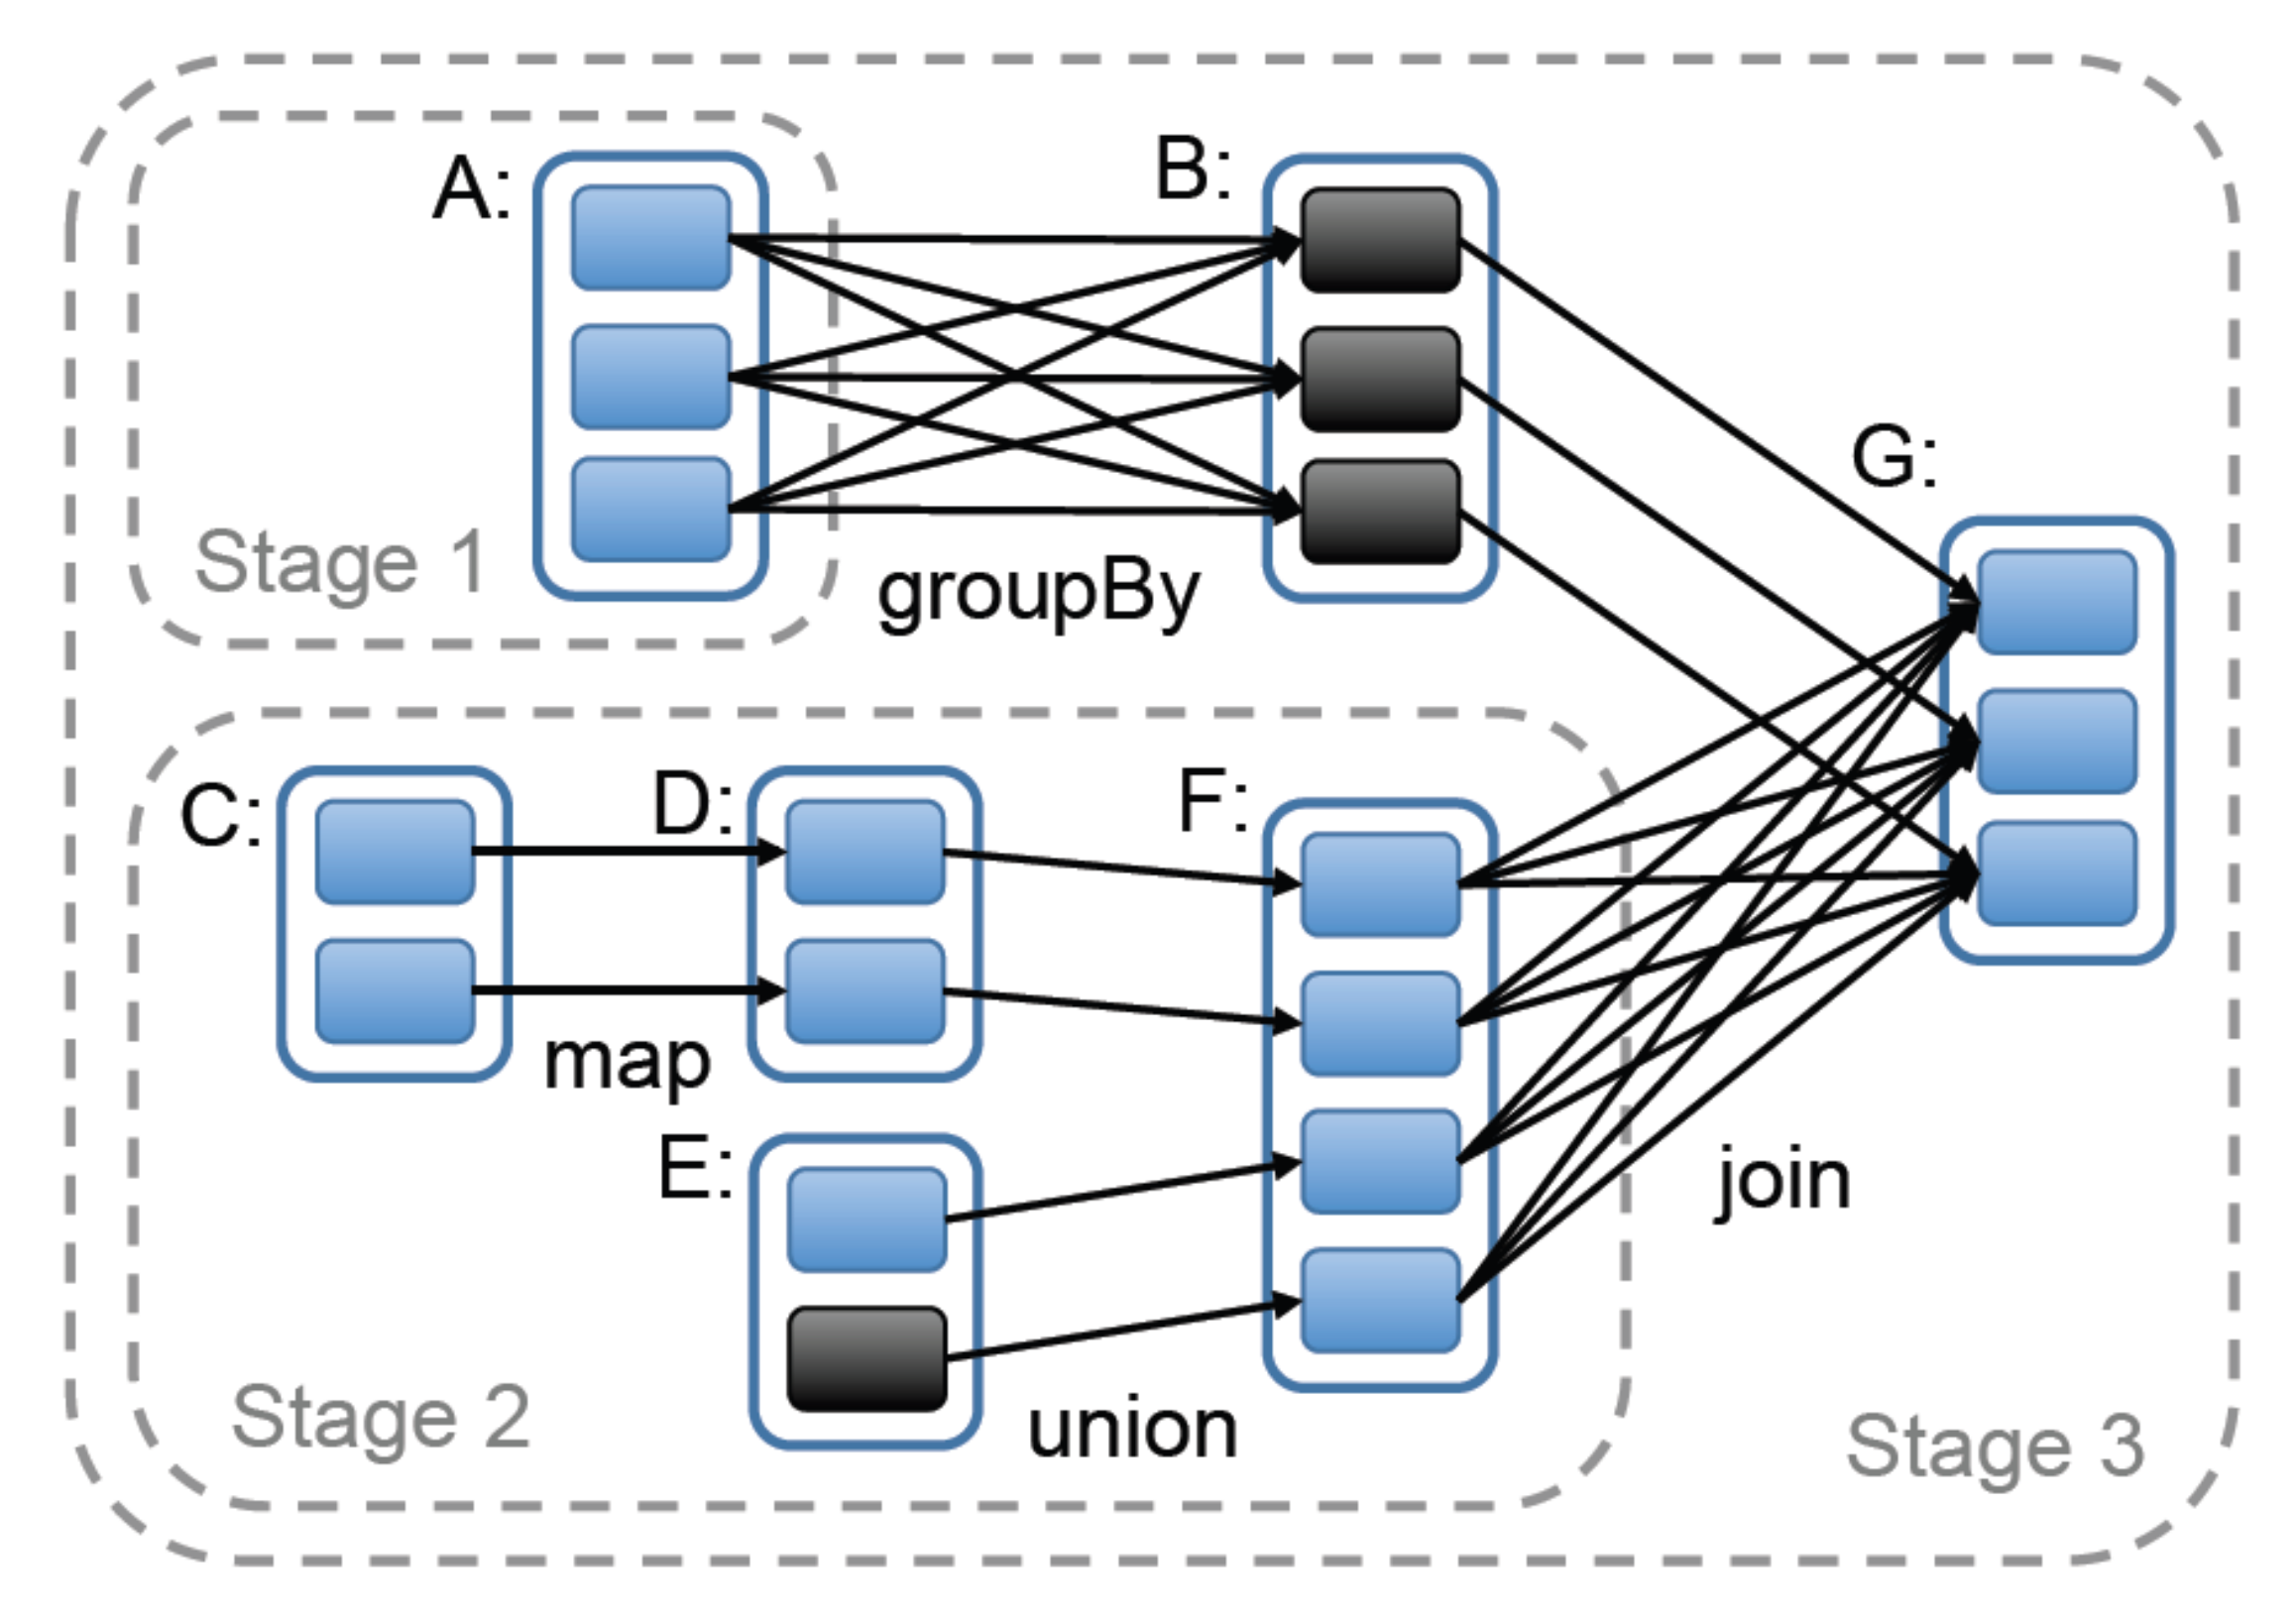
\includegraphics[width=0.5\linewidth]{Figures/partition-tracking.png}
    \end{figure}
\end{frame}


\begin{frame}[fragile]{Parallelizing SGD}
    \begin{enumerate}
        \item Master broadcasts model parameters to workers
        \item Each worker runs SGD on its subset for $\tau=50$ iterations
        \item Worker model parameters collected and averaged on master
    \end{enumerate}

    \begin{scalacode}
var trainData = loadData(...)
var trainData = preprocess(trainData).cache()
var nets = trainData.foreachPartition(data => {
    var net = Net(netParams)
    net.setTrainingData(data)
    net
})
var weights = initialWeights(...)
for (i <- 1 to 1000) {
    var broadcastWeights = broadcast(weights)
    nets.map(net => net.setWeights(broadcastWeights.value))
    weights = nets.map(net => {
        net.train(50)
        net.getWeights()
    }).mean() // an average of WeightCollection objects
}
    \end{scalacode}
\end{frame}


\begin{frame}{SparkNet Architecture}
\begin{figure}[htpb]
    \centering
    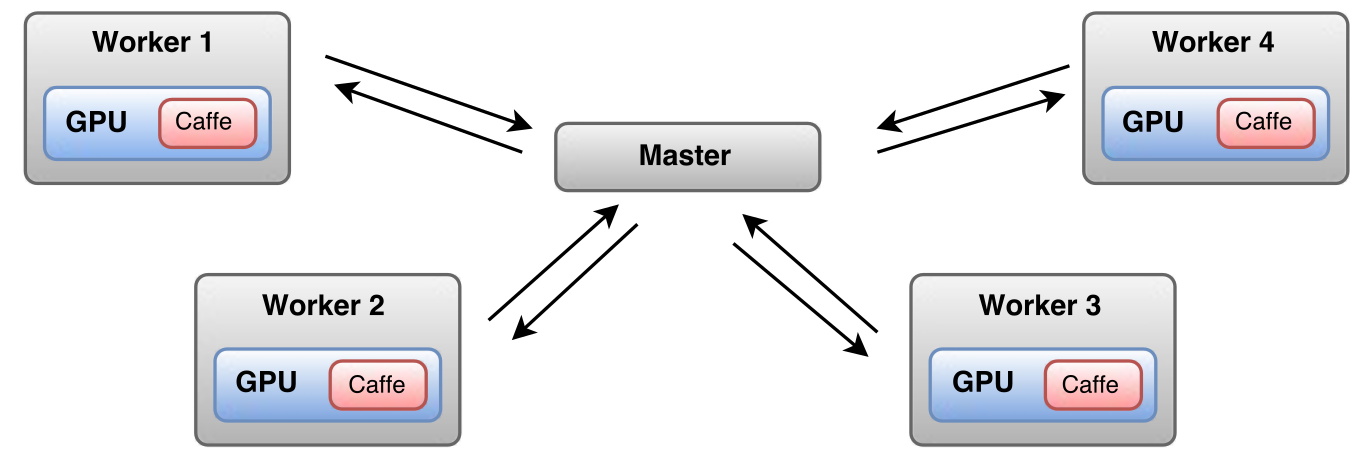
\includegraphics[width=0.8\linewidth]{Figures/arch.png}
\end{figure}
\end{frame}

\section{Architecture Discussion}

\begin{frame}{Concerns in distributed optimization: communication}
    \begin{block}{Inter-machine communication bottleneck}
        Worker machines must frequently read and write the global shared
        parameters.
    \end{block}


    \begin{alertblock}{Question: How does SparkNet's $\tau=50$ affect
        communication? Convergence rate?}
        \pause
        \begin{itemize}
            \item Communication once every $\tau$ instead of every single SGD iteration
            \item Workers obtain parameter estimates more biased to own partition
        \end{itemize}
    \end{alertblock}
\end{frame}

\begin{frame}{Concerns in distributed optimization: stragglers}
    \begin{block}{The straggler problem}
        Many algorithms require synchronization barriers, which are rate-limited
        by the slowest machines.
    \end{block}

    \begin{alertblock}{Question: Why might some machines be slower than others?}
        \pause
        \begin{itemize}
            \item Imbalanced workload partitioning
            \item Network congestion
            \item Other processes in multi-tenant environments
        \end{itemize}
    \end{alertblock}
\end{frame}

\begin{frame}{Addressing the straggler problem: asynchronous SGD}
    \textbf{Not addressed by SparkNet}, but an active research area:
    \begin{itemize}
        \item HogWild! -- Correctness guaranteess \cite{recht2011hogwild}
        \item Parameter server -- Distributed implementation \cite{ho2013more},
            flexible consistency models in V3 \cite{li2013parameter}
    \end{itemize}

    \begin{figure}[htpb]
        \centering
        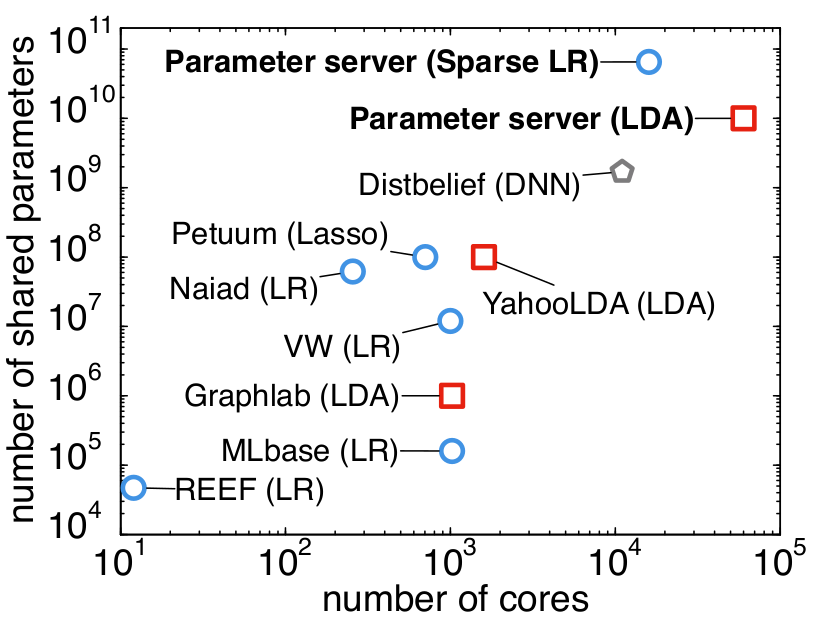
\includegraphics[width=0.5\linewidth]{Figures/parameter-servers.png}
    \end{figure}
\end{frame}

\section{Results}

\begin{frame}[t]{Tuning $\tau$}
    \begin{itemize}
        \item All experiments on EC2 g2.8xlarge nodes
        \item AlexNet \cite{krizhevsky2012imagenet}
        \item $K=5$ workers
    \end{itemize}
    \begin{figure}[htpb]
        \centering
        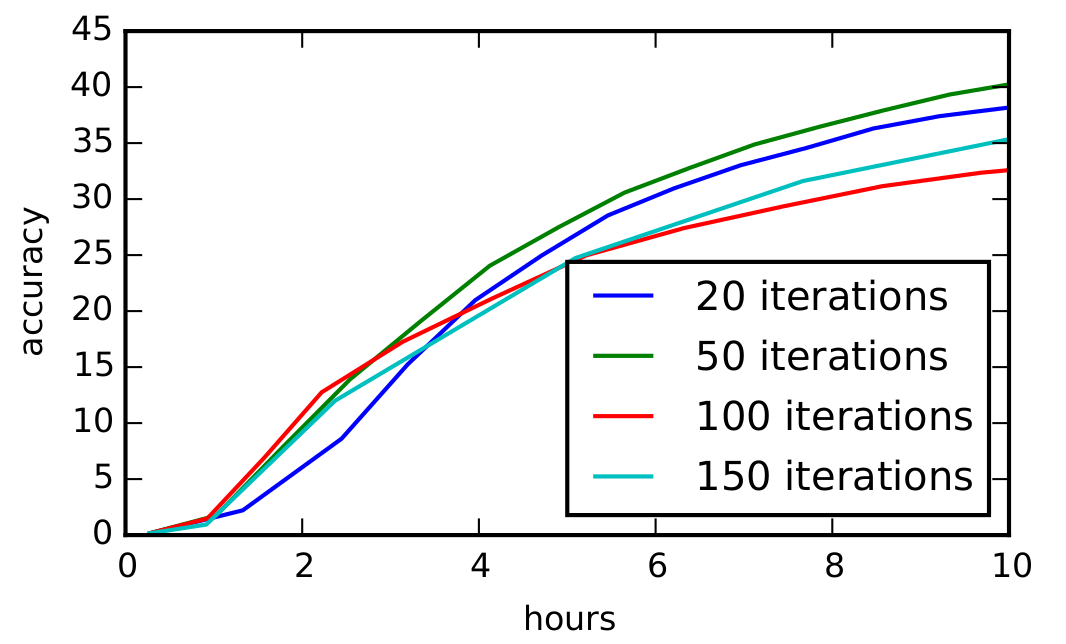
\includegraphics[width=0.6\linewidth]{Figures/tau-acc.png}
    \end{figure}
\end{frame}

\begin{frame}[t]{Training curves}
    \begin{columns}
        \begin{column}{0.5\textwidth}
            \begin{itemize}
                \item AlexNet \cite{krizhevsky2012imagenet}
                \item 8 layer CNN, ILSVRC2010
                \item $\tau=50$
            \end{itemize}
            \begin{figure}[htpb]
                \centering
                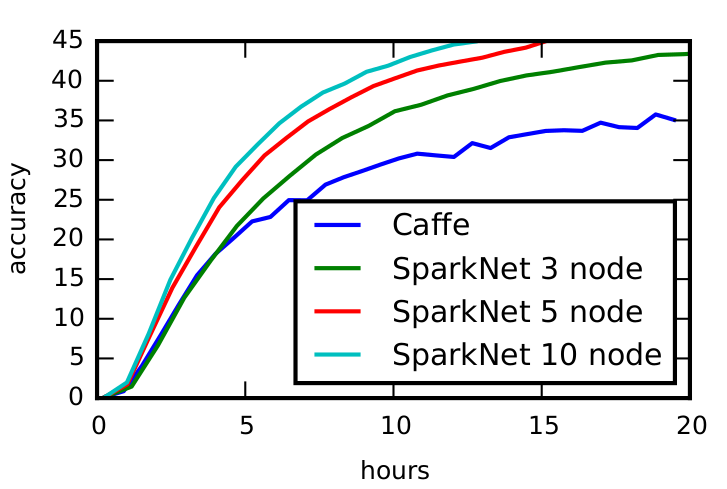
\includegraphics[width=\linewidth]{Figures/single-gpu.png}
            \end{figure}
        \end{column}
        \begin{column}{0.5\textwidth}
            \begin{itemize}
                \item GoogLeNet \cite{szegedy2015going}
                \item 22 layer CNN, ILSVRC2014
                \item $\tau=50$
            \end{itemize}
            \begin{figure}[htpb]
                \centering
                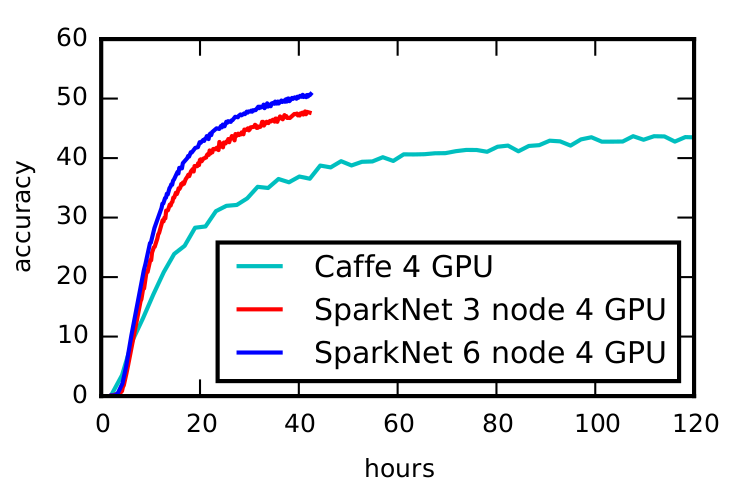
\includegraphics[width=\linewidth]{Figures/multi-gpu.png}
            \end{figure}
        \end{column}
    \end{columns}
\end{frame}

\begin{frame}{Speedups relative to single-GPU Caffe}
    \begin{figure}[htpb]
        \centering
        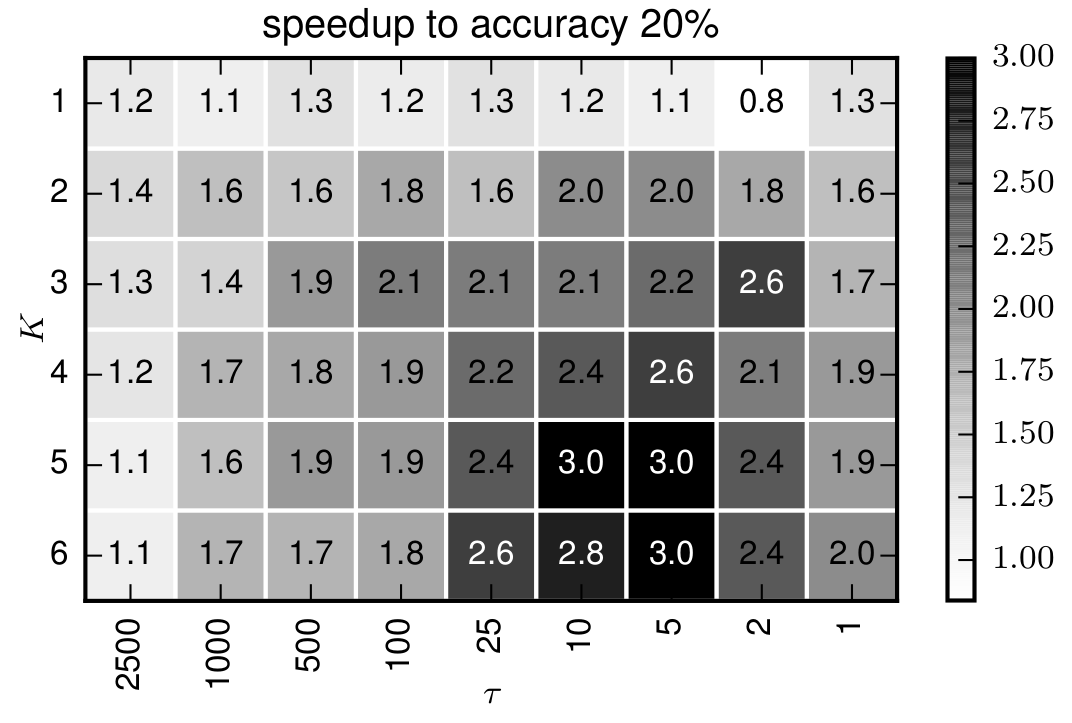
\includegraphics[width=0.6\linewidth]{Figures/grid.png}
    \end{figure}
    \begin{itemize}
        \item Why is $K=1$ largely unaffected by $\tau$?
        \item Why does performance deteriorate with increasing $K$?
            Increasing $\tau$?
    \end{itemize}
\end{frame}

\section{Discussion}

\begin{frame}[t]{Related work}
    \begin{itemize}
        \item Distbelief \cite{dean2012large} 
            \begin{itemize}
                \item Both data-parallel and \textbf{model-parallel} DNNs
                \item Asynchronous (downpour SGD) and batch (sandblaster L-BFGS
                \item Google Borg CPU cluster
            \end{itemize}
        \item FireCaffe \cite{iandola2015firecaffe}
            \begin{itemize}
                \item Caffe parameter server
                \item Cray GPU cluster
                \item \textbf{SoA $47\times$ speedup} training GoogLeNet
                    on 128 GPUs
            \end{itemize}
        \item Yahoo/CaffeOnSpark \cite{caffe-on-spark}
            \begin{itemize}
                \item Infiniband/ethernet for GPU parameter exchange
                \item \textbf{Spark and EC2 integration}
            \end{itemize}
    \end{itemize}
\end{frame}

\begin{frame}[t]{Conclusion}
    \begin{itemize}
        \item Contributions
            \begin{itemize}
                \item Data-parallel integration between a popular deep CNN tool
                    (\emph{Caffe}) and a general-purpose cluster computing
                    (\emph{Spark}) framework
                \item Empirical studies on $\tau$ and $K$
            \end{itemize}
        \item Criticisms
            \begin{itemize}
                \item Does not solve straggler problem: synchronization
                    barrier at each parameter collection step
                \item No comparison against related work
                \item Experiments are too small (10 nodes max)
            \end{itemize}

        \item Future work
            \begin{itemize}
                \item Mathematical analysis of $\tau$'s effects
                    on learning convergence
                \item Lock-free parameter updates (will require
                    extending Spark)
            \end{itemize}
    \end{itemize}
\end{frame}

\begin{frame}[allowframebreaks]
    \frametitle{References}
    \bibliographystyle{amsalpha}
    \nocite{*}
    \bibliography{refs.bib}
\end{frame}

\end{document}
